%--------------------------------------------------------------------------------------------------
% 
\chapter{Feature Selection Using Multi-Objective Optimization}
\label{ch:feature-selection}
%--------------------------------------------------------------------------------------------------

\epigraph{Natural selection is the preservation of favored races in the struggle for life.}{\textit{Charles Darwin}}

\begin{quote}
This chapter presents the paper titled \textit{FASTENER feature selection for inference from earth observation data} by Filip Koprivec, Klemen Kenda and Beno Šircelj published in Entropy journal (IF 2020: 2.524)~\cite{koprivec:2020:fastener}.
Filip Koprivec and Klemen Kenda share the first authorship of the paper.
Klemen Kenda contributed to conceptualization and methodology, validation, writing and also to project administration and funding acquisition. 
Klemen Kenda was supervising the work of the other co-authors.
\end{quote}

Feature selection represents a crucial step in optimizing the performance of the model.
Based on the evaluation criterion, the feature selection methods are divided into filter and wrapper methods.
Filter methods utilize the statistical performance of the data it trains for feature evaluation and do not have a relation to the learning algorithm used.
On the other hand, wrapper methods use the training accuracy of learning algorithms.
Algorithms can, therefore, capture more specific behavior at the expense of computational complexity.
For wrapper algorithms, feature selection represents a search in the feature space.
The task of finding a minimal feature set that yields the best possible model results is proven to be an NP problem~\cite{hua:2009:performance}.

Wrapper algorithms employ different search algorithms for feature selection: complete search, heuristic search, random search \cite{jia:2022:feature}.
A complete search can find the optimal solution; however it often demands relatively large computational requirements.
To find the optimal feature subset, the $M$-feature combinations of $N$ original features must be searched. 
Therefore, in most practical situations, an exhaustive search cannot be achieved~\cite{jia:2022:feature}.

FASTENER algorithm belongs to the family of random search approaches.
It was originally developed to be used in land-use classification based on earth observation data, however, we have shown that the algorithm performs very well also on several other use cases, including environmental and biological datasets.
FASTENER exploits entropy-based measures, such as mutual information in the crossover phase of the iterative genetic approach. 
FASTENER outperforms other multi-objective wrapper methods in terms of converging to a (near) optimal subset of features more quickly.

We evaluate the performance of wrapper methods with an area under (Pareto) front ($\textit{AUF}$), where the front is represented with $F_1$ scores of an optimal $k$ selected features for a particular classification problem.
FASTENER outperforms the POSS~\cite{qian:2015:poss} and FS-SDS~\cite{alhakbani:2017:fs-sds} algorithms in Earth observation data sets with an average $\textit{AUF}$ of $0.71$, compared to $0.66$ and $0.62$ for POSS and FS-SDS, respectively.
FASTENER also produces surprisingly good results in the benchmark datasets for feature selection~\cite{li:2017:feature}, where its average $\textit{AUF}$ score is better than the FS-SDS $\textit{AUF}$ score in almost all, except one out of 25 datasets.
On average difference between $\textit{AUF}$ scores betweeen FS-SDS and FASTENER in $0.08$, where FASTENER needed more than $2.5$-times less model evaluations.
Compared to DT-forward algorithm~\cite{guyon:2003:dt-forward}, FASTENER yields better results in nine out of 25 benchmark datasets.
It is worth mentioning that FASTENER requires on average $2$ to $5$ times fewer model evaluations than DT-forward, while achieving comparable or better results.

Finally, FASTENER demonstrates superior classification accuracy when compared with similarity and information theory-based techniques typically applied in Earth observation scenarios.
FASTENER was also tested on open feature selection datasets and compared with state-of-the-art methods. 
It achieves comparable results, however, with fewer model evaluations.
FASTENER can be used in any supervised machine learning scenario.

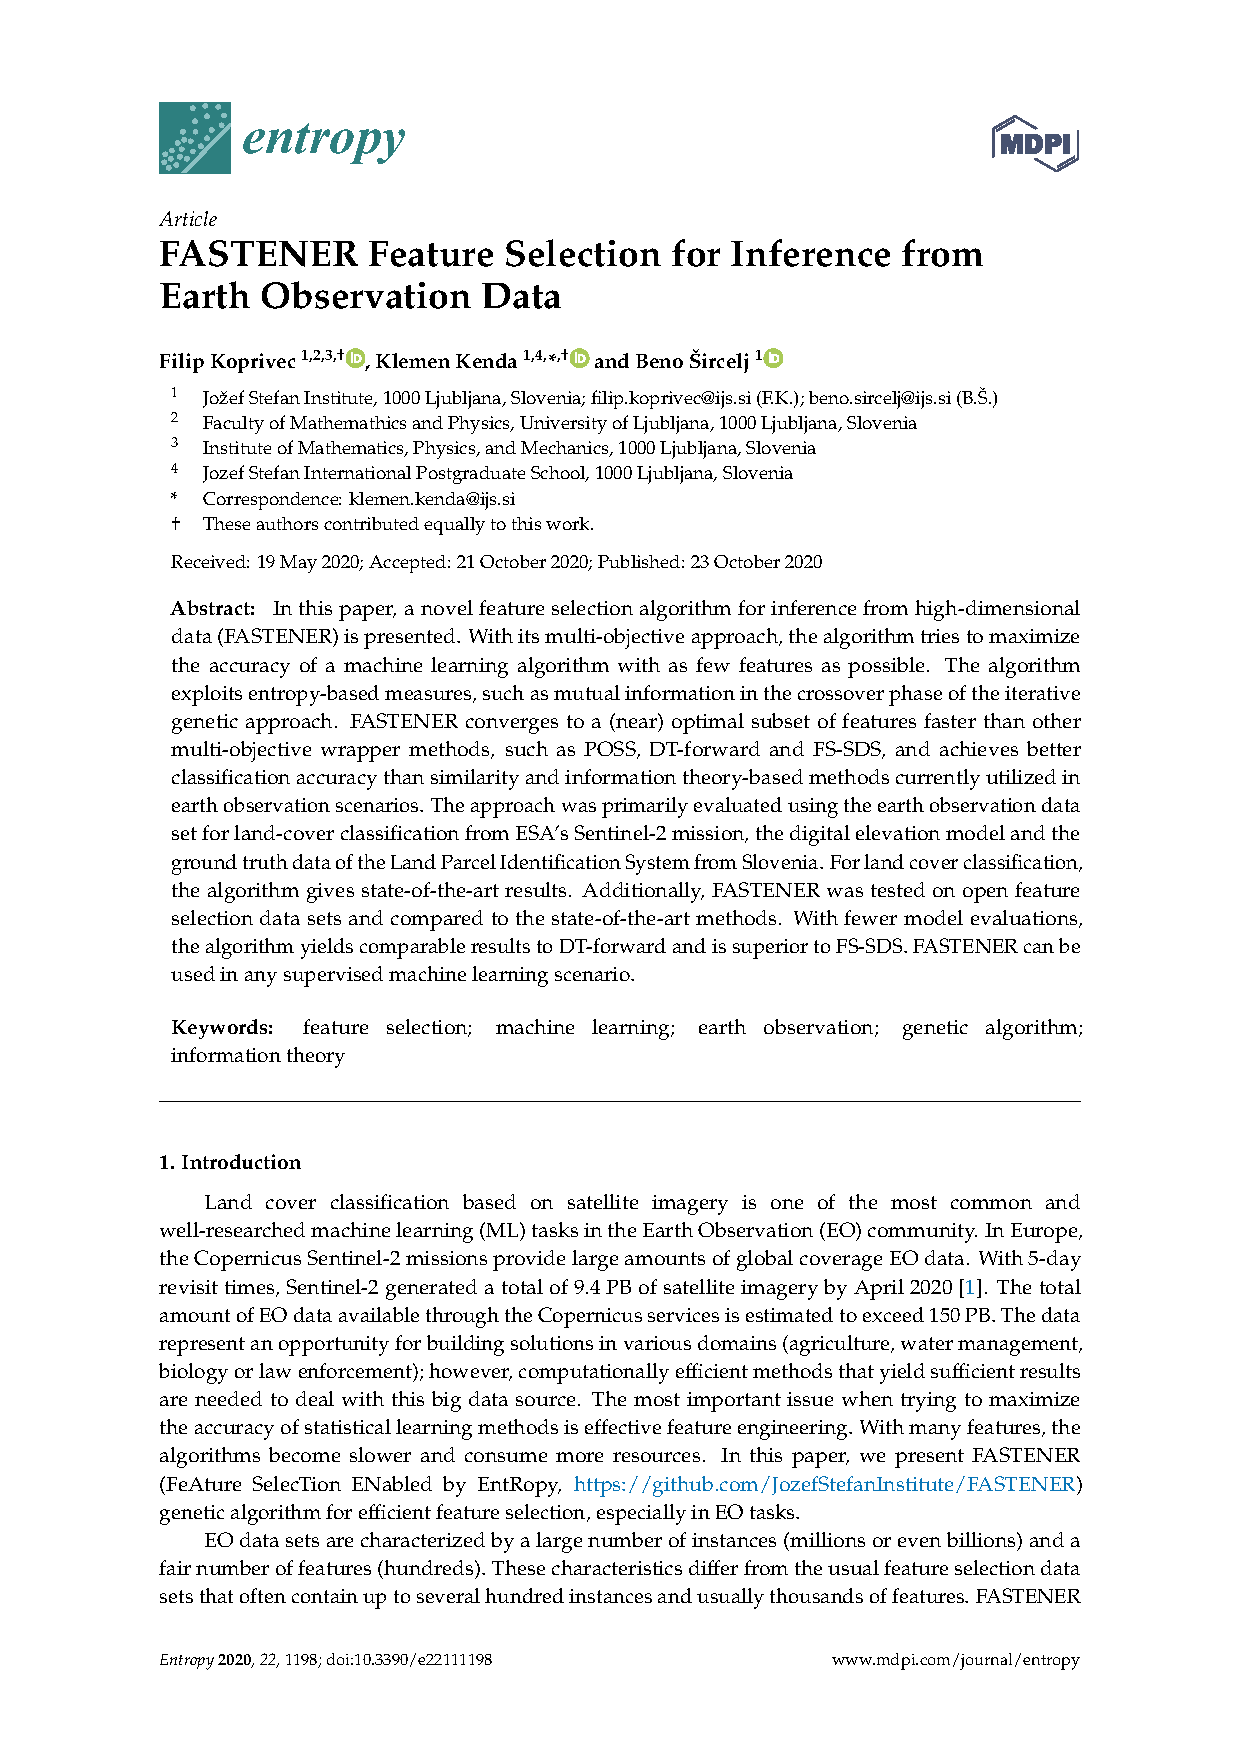
\includepdf[pages=-]{papers/fastener.pdf}
